\documentclass[conference]{IEEEtran}
\IEEEoverridecommandlockouts
\usepackage{cite}
\usepackage{amsmath,amssymb,amsfonts}
\usepackage{graphicx}
\usepackage{textcomp}
\usepackage{xcolor}
\usepackage{booktabs}
\usepackage{multirow}
\usepackage{url}
\usepackage{array}

% Decision states are labels, not products of variables: keep them upright.
\newcommand{\dstate}[1]{\ensuremath{\mathrm{#1}}}
% Indicator function. \mathbb{1} is not available in msbm (it renders as a
% stray relation symbol), so the indicator is set with a bold upright 1.
\newcommand{\ind}{\mathbf{1}}

\begin{document}

\title{Uncertainty-Aware Multimodal Evidence Fusion for
Vessel-Associated Subsea Cable Disturbance Assessment}

\author{
\IEEEauthorblockN{Dr.A.Syed Musthafa\IEEEauthorrefmark{1}}
\IEEEauthorblockA{Department of Information Technology\\
M Kumarasamy College of Engineering\\
Karur, India\\
sathiyanathans@mkce.ac.in}
\and
\IEEEauthorblockN{Muthukrishnan C}
\IEEEauthorblockA{Department of Information Technology\\
M Kumarasamy College of Engineering\\
Karur, India\\
muthukrishnanchellamuthu8893@gmail.com}
\and
\IEEEauthorblockN{Muthuvel Mukesh K}
\IEEEauthorblockA{Department of Information Technology\\
M Kumarasamy College of Engineering\\
Karur, India\\
muthuvelmukesh0609@gmail.com}
\and
\IEEEauthorblockN{Shanmugavel M}
\IEEEauthorblockA{Department of Information Technology\\
M Kumarasamy College of Engineering\\
Karur, India\\
mshanmugavel065@gmail.com}
\thanks{\IEEEauthorrefmark{1}Corresponding author.}
}

\maketitle

\begin{abstract}
Subsea power and telecommunication cables support critical global communications and energy distribution, but detecting an anomalous seafloor vibration does not establish whether a maritime vessel caused it or whether the cable sustained physical damage. Conventional monitoring systems frequently conflate acoustic disturbances with surface vessel threats, producing excessive false alarms or vulnerability to vessel-side telemetry spoofing. This paper develops an uncertainty-aware multimodal evidence fusion framework that explicitly decouples physical disturbance detection, spatio-temporal association, vessel kinematics, sensor health evaluation, and counter-evidence assessment into distinct evidence streams. These streams are combined through a graded, fail-closed decision hierarchy that outputs operational states \dstate{T0}--\dstate{T3} alongside a degraded-evidence state \dstate{TX}. The framework is evaluated across three submarine distributed acoustic sensing (DAS) deployments: an Automatic Identification System (AIS)-linked container-ship transit in the North Sea (Marlinks), an unperturbed deep-sea background recording in the Mediterranean (EMSO Western Ionian), and a 27.625-day continuous Arctic deployment (Dryad Oliktok). On the Marlinks dataset, the DAS channel separates 1~km corridor incursions with an area under the receiver operating characteristic curve (AUC) of $0.959$ (95\% CI $[0.887, 1.000]$), with acoustic power tracking vessel distance at Spearman $\rho=-0.948$. In unperturbed conditions, the framework generated zero false escalations across 85/85 deep-sea background windows and all 215 multi-week Arctic windows, exhibiting a stable baseline (drift $+0.0188/\mathrm{hr}$, $p=0.8037$) that tracked independent sea-surface wave height. Across four vessel-side AIS manipulation attack families spanning five severity levels, the adversarial evasion rate was $0.0$. As an intentional design trade-off, the framework achieves a lower escalation F1 score ($0.462$ on real transit data, $0.235$ in 2{,}200 controlled simulation trials) than simple weighted fusion ($0.824$ and $0.333$, respectively), prioritizing fail-closed security over unconstrained escalation recall. Mean end-to-end processing latency is 8.289~ms, confirming compatibility with real-time operational monitoring.
\end{abstract}

\begin{IEEEkeywords}
subsea cable protection, distributed acoustic sensing, Automatic
Identification System, multimodal sensor fusion, uncertainty estimation, critical infrastructure,
adversarial robustness, environmental robustness, reproducibility
\end{IEEEkeywords}

\section{Introduction}

Subsea optical telecommunication and high-voltage power cables transport international data and electrical energy across oceanic basins. Mechanical damage inflicted by surface maritime operations---predominantly anchor dragging, bottom-trawl gear entanglement, and uncoordinated maneuvering---accounts for the majority of non-geological cable faults. While automated surveillance is critical to mitigate service disruptions, isolating threat-bearing human activity from acoustic seabed measurements presents severe operational challenges.

Vibrations recorded by optical fibers along the seafloor originate from multiple concurrent sources: direct vessel-hull acoustic coupling, benthic mechanical contact, oceanographic hydrodynamic forcing (such as surface gravity waves and microseisms), and optical interrogator noise. A physical signal deviation alone does not identify the generating mechanism. We therefore structure the disturbance assessment problem around three distinct inferential stages:
\begin{equation}
\text{Detection} \neq \text{Association} \neq \text{Attribution}.
\label{eq:principle}
\end{equation}
Physical \emph{detection} determines whether an anomalous energetic deviation occurred on the fiber array. Spatio-temporal \emph{association} tests whether that disturbance coincides in space and time with known external vessel movements. Causal \emph{attribution} evaluates whether the assembled multimodal evidence warrants assigning responsibility to a specific external craft or operational mechanism.

Conflating these stages undermines operational safety. As demonstrated in Section~\ref{sec:real-results}, acoustic strain from a transiting cargo ship propagates over 1.5~km through seabed sediments. An uncorroborated physical detector triggers continuously during distant transit, producing a recall of 1.000 but a precision of only 0.526 within a 1~km protection corridor.

Compounding this physical ambiguity, vessel-side reporting through the Automatic Identification System (AIS) operates over unauthenticated radio links susceptible to intentional GPS spoofing, transponder suppression, and coordinate falsification. An evidence-fusion system that naively trusts AIS broadcasts can be misled into dismissing genuine physical threats or generating false alarms during legitimate operations. Robust cable monitoring therefore requires explicitly bounding both natural environmental variation and vessel-side adversarial uncertainty.

\subsection{Scope and Validation Status}
\label{sec:scope-detail}

To maintain scientific rigor, this paper reports experimental outcomes strictly for executed modules, validated through traceable cryptographic hashes and reproducibility manifests. The investigation defined four validation components:
(i) controlled synthetic simulation across 22 benchmark scenarios (2{,}200 trials);
(ii) empirical validation on real submarine DAS and AIS transit records;
(iii) long-duration environmental robustness validation against independent Arctic oceanographic moorings; and
(iv) physical hardware-in-the-loop validation using ESP32--MPU6050 sensor nodes.

Components (i), (ii), and (iii) were fully executed and are reported with exact numerical metrics. Component (iv) was not physically constructed; Section~\ref{sec:hardware} details its proposed architectural scope, target empirical measurements, and boundary conditions. Table~\ref{tab:status} outlines the validation status across all components.

\begin{table}[!t]
\caption{Validation Status of the Evaluated and Proposed Framework Components}
\label{tab:status}
\centering
\footnotesize
\setlength{\tabcolsep}{3pt}
\begin{tabular}{@{}>{\raggedright\arraybackslash}p{0.34\columnwidth}>{\raggedright\arraybackslash}p{0.30\columnwidth}>{\raggedright\arraybackslash}p{0.26\columnwidth}@{}}
\toprule
Component & Evidence / Scope & Status \\
\midrule
Controlled simulation (S01--S22) & 2{,}200 seeded trials & \textbf{EXECUTED} \\
Real DAS + AIS transit (Dataset A) & 60 windows, 250 ch & \textbf{EXECUTED} \\
Real DAS background (Dataset B) & 105 windows, 2{,}963 ch & \textbf{EXECUTED} \\
Real DAS environmental (Dataset C) & 215 windows, 183 ch, 27.6~d & \textbf{EXECUTED} \\
Adversarial sweep on vessel AIS & 4 families $\times$ 5 sev. & \textbf{EXECUTED} \\
ESP32--MPU6050 testbed & Bench hardware build & FUTURE (Sec.~\ref{sec:hardware}) \\
Multi-vessel / damaged cable DAS & External incident logs & NOT EXECUTED \\
\bottomrule
\end{tabular}
\end{table}

The primary contributions of this paper are:
\begin{enumerate}
\item A multimodal evidence fusion architecture that decouples physical disturbance detection from spatio-temporal association, vessel behavior, sensor health, and uncertainty estimation, employing a fail-closed graded decision model (\dstate{T0}--\dstate{T3}, \dstate{TX}).
\item A spatially coherent detection statistic whose operational threshold is calibrated on an independent deep-sea background record rather than evaluation splits, establishing a verified baseline false-alarm rate.
\item An adversarial cross-consistency check that contrasts DAS-derived range inversion against vessel-broadcast AIS ranges, preventing vessel-side falsification from silently forcing benign classifications.
\item Multi-environment empirical validation across three submarine DAS deployments (Belgian North Sea, Western Ionian Sea, and Arctic Beaufort Sea) spanning over 27.6 days of continuous acoustic recording, verifying spatial strain decay, deep-sea stationarity, and hydrodynamic wave coupling.
\item Complete decision-rule backward compatibility across 22 benchmark scenarios (22/22 identical decisions) under an updated reliability-first decision hierarchy, resolving quiet-baseline misclassifications.
\item A documented accounting of conservative design trade-offs: at reference thresholds, the full framework yields lower escalation F1 than unconstrained weighted fusion across both simulated and real data, reflecting intentional fail-closed safety.
\end{enumerate}

\section{Related Work}

\subsection{Subsea Cable Monitoring and Sensing}
Structural health monitoring of underwater power and telecommunication cables has historically relied on Remotely Operated Vehicles (ROVs), sensing coil arrays, and optical time-domain reflectometry \cite{b1,b2,b3,b4}. While effective for post-fault localization and scheduled maintenance, these modalities cannot provide continuous, automated surveillance of proximate surface threats.

\subsection{Submarine Distributed Acoustic Sensing (DAS)}
Distributed acoustic sensing (DAS) leverages coherent optical time-domain reflectometry ($\Phi$-OTDR) to turn standard subsea optical fibers into dense arrays of dynamic strain sensors spanning tens of kilometers. Prior investigations have demonstrated submarine DAS for seismic observation, ocean wave monitoring, and opportunistic vessel acoustic tracking \cite{b11,b12,b13,b14,b15}. These studies largely treat raw acoustic processing, beamforming, or inverse acoustic ranging as isolated objectives. By contrast, our work incorporates DAS strain sensing as one physical input within a broader, uncertainty-aware evidence fusion architecture.

\subsection{AIS Integrity and Maritime Anomaly Detection}
Broadcast kinematics from the Automatic Identification System (AIS) are widely used for maritime collision avoidance and traffic tracking \cite{b5,b6,b7}. Because AIS broadcasts are unencrypted and lack cryptographic origin verification, transponders can be powered down, spoofed with false Maritime Mobile Service Identity (MMSI) headers, or manipulated through coordinate offsets. As a result, AIS data cannot be treated as an authoritative oracle; broadcasts must be corroborated against independent physical sensor channels.

\subsection{Evidence Fusion under Conflict and Uncertainty}
Classical combination rules, including Dempster--Shafer and Dezert--Smarandache theories, formalize belief assignment across disparate sensor sources. In high-conflict regimes, however, unweighted combination rules can yield erratic or non-intuitive decisions \cite{b8,b9,b10}. Modern extensions employ reliability weighting, distance-based conflict discounting, and explicit uncertainty boundaries. We adopt these principles to link sensor availability, hardware health, and adversarial consistency checks within a fail-closed decision hierarchy.

\section{Problem Formulation}

Let $X = \{X_1, \ldots, X_N\}$ represent multimodal observations collected across temporal sliding windows, where each observation possesses a sensor tag and timestamp. We evaluate four competing hypotheses:
\begin{align}
H_1&: \text{vessel-associated subsea disturbance}, \\
H_2&: \text{environmental / hydrodynamic disturbance}, \\
H_3&: \text{non-vessel mechanical seabed disturbance}, \\
H_4&: \text{sensor degradation or interrogator fault}.
\end{align}
The decision rule maps the evidence space into a discrete operational state:
\begin{equation}
D = f(E^{+}, E^{-}, H, U, A),
\end{equation}
where $E^{+}$ represents supporting evidence, $E^{-}$ represents counter-evidence, $H$ is the hypothesis space, $U \in [0, 1]$ is quantified uncertainty, and $A \in [0, 1]$ represents sensor data availability.

\subsection{Adversarial Threat Model}
Let $X_{H_1}$ denote genuine observations generated during a true vessel-associated interaction. An adversary seeking to conceal their presence manipulates the vessel-side communication stream within an adversarial budget $\Omega$, producing perturbed observations $\tilde{X}$. The threat model addresses four vessel-side attack families:
(i) range inflation (transmitting coordinates artificially distant from the cable);
(ii) transponder suppression (omitting transmission bursts);
(iii) timestamp manipulation (injecting artificial transmission latencies); and
(iv) combined multi-vector evasion.

Physical tampering with the subsea fiber, optical interrogator firmware compromise, and terrestrial communications network intrusion are explicitly outside this threat model. The core safety requirement is that genuine incursions under attack must not collapse to baseline:
\begin{equation}
\forall \tilde{X} \in \Omega(X_{H_1}): D(\tilde{X}) \neq \dstate{T0}.
\label{eq:safety}
\end{equation}
The framework does not guarantee that every adversarial scenario escalates to high-severity alert \dstate{T3}. Instead, when evidence is degraded or severely conflicted, the decision must default to \dstate{TX} (degraded/conflicted evidence) rather than erroneously resolving to normal baseline \dstate{T0}.

\section{Proposed Framework}

The architecture (Fig.~\ref{fig:architecture}) processes raw DAS phase strain rates and AIS kinematic broadcasts through separate feature extraction pipelines before performing spatio-temporal association, sensor health validation, adversarial consistency verification, uncertainty estimation, and graded decision assignment:
\begin{equation}
C_P \rightarrow (C_S, C_T, C_B) \rightarrow C_A \rightarrow R \rightarrow U \rightarrow D,
\end{equation}
where $C_P$ denotes physical disturbance confidence; $C_S, C_T, C_B$ represent spatial, temporal, and behavioral association confidences; $C_A$ is composite association confidence; $R$ is fused evidence reliability; $U$ is composite uncertainty; and $D$ is the final decision state.

\begin{figure}[!t]
\centering
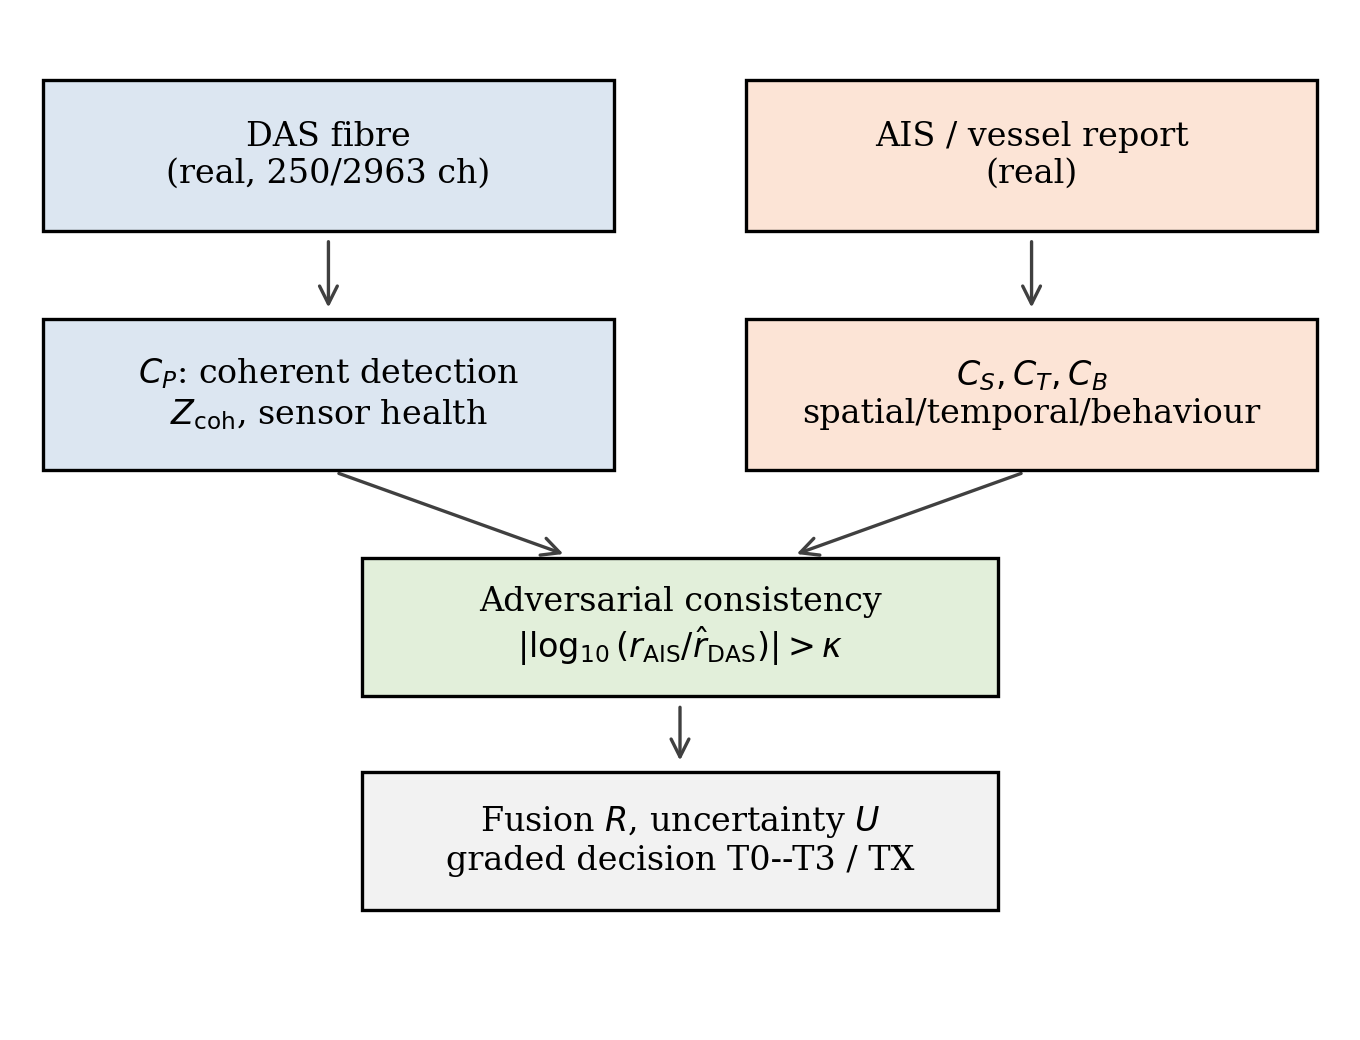
\includegraphics[width=0.46\textwidth]{figs/fig_architecture.png}
\caption{Processing architecture. The optical DAS strain pipeline and AIS vessel telemetry remain strictly separated until the adversarial consistency check, preventing vessel-side falsification from corrupting physical detection.}
\label{fig:architecture}
\end{figure}

\subsection{Physical Disturbance Detection}
For spatial channel $i$, the primary window feature is the root-mean-square (RMS) strain amplitude $A_i = \sqrt{\frac{1}{n}\sum_s x_{i,s}^2}$. Per-channel mean $\mu_i$ and standard deviation $\sigma_i$ are estimated over quiescent baseline periods, yielding the standardized anomaly score $z_i = |A_i - \mu_i| / \sigma_i$.

Because localized fading spikes or optical noise excursions can cause extreme $z$-scores on individual fiber channels, single-channel thresholding cannot reliably govern false-alarm rates across thousands of sensing channels. Seabed vibrations generated by heavy maritime activity couple elastically into the sediment and excite multiple adjacent fiber channels. We therefore define the cable-level physical detection statistic as the maximum $L$-channel spatial moving average:
\begin{equation}
Z_{\mathrm{coh}} = \max_j \frac{1}{L}\sum_{i=j}^{j+L-1} z_i,
\qquad
C_P = \mathrm{sig}\!\left(\frac{Z_{\mathrm{coh}} - \tau_P}{k_P}\right),
\label{eq:zcoh}
\end{equation}
where $\mathrm{sig}(v) = 1/(1+e^{-v})$. The spatial window length $L$ and detection threshold $\tau_P$ are calibrated exclusively on independent background data disjoint from evaluation splits.

\subsection{Spatial and Temporal Association}
Spatial proximity confidence is $C_S = \max(0, 1 - d/d_{\max})$, where $d$ is the estimated distance from the vessel to the cable array and $d_{\max}$ is the surveillance corridor radius. Temporal synchronization confidence is $C_T = \max(0, 1 - |\Delta t| / t_{\max})$, where $\Delta t$ is the latency between acoustic energy onset and the vessel's closest point of approach (CPA) time. Rather than selecting an arbitrary temporal window, $t_{\max}$ adapts dynamically to vessel kinematics as $t_{\max} = d_{\max} / v$, where $v$ is vessel speed over ground.

\subsection{Vessel Behavior and Sensor Health Weighting}
Behavioral risk confidence is evaluated over normalized kinematic features $\phi_k(v)$ (speed anomalies, rate of turn, course changes): $C_B = \mathrm{sig}\!\left(\sum_k b_k \phi_k(v)\right)$. Composite association confidence combines these components: $C_A = \alpha C_S + \beta C_T + \gamma C_B$, with $\alpha + \beta + \gamma = 1$.

Sensor health $H_i = 1 - \max_k(\rho_k \psi_k(i))$ tracks hardware integrity across degradation indicators $\psi_k$ (flatlined channels, optical saturation, non-finite values). Incorporating data availability $V_i \in [0, 1]$ and assigned weights $w_i$, the fused evidence reliability score is:
\begin{equation}
R = \frac{\sum_i w_i H_i V_i C_i}{\sum_i w_i H_i V_i + \epsilon}.
\end{equation}
This formulation prevents degraded or offline sensors from artificially inflating detection confidence.

\subsection{Adversarial Range Consistency Check}
A vessel falsifying its AIS stream to hide cable proximity displaces its reported range $r_{\mathrm{AIS}}$ while leaving seabed acoustic strain unaltered. The DAS array provides an independent physical range estimate $\hat{r}_{\mathrm{DAS}}$. The consistency check fires when the vessel-reported distance substantially exceeds the acoustic estimate during an active physical disturbance:
\begin{equation}
\log_{10}\!\left(\frac{r_{\mathrm{AIS}}}{\hat{r}_{\mathrm{DAS}}}\right) > \kappa
\ \wedge\ C_P \geq \theta_P \;\Rightarrow\; \dstate{TX}.
\label{eq:consistency}
\end{equation}
Routing these discrepancies directly to \dstate{TX} flags deliberate manipulation rather than allowing silent evasion to \dstate{T0}.

\subsection{Uncertainty Quantification and Graded Decision Engine}
\label{sec:decision-engine}

Four uncertainty metrics (missing telemetry $U_{\mathrm{miss}}$, sensor degradation $U_{\mathrm{health}}$, evidence divergence $U_{\mathrm{conf}}$, and association ambiguity $U_{\mathrm{assoc}}$) are combined into a composite uncertainty score: $U = \sum_{j=1}^4 \lambda_j U_j$.

The decision hierarchy applies reliability-first gating to ensure fail-closed safety without misclassifying quiet baselines:
\begin{equation}
T =
\begin{cases}
\dstate{TX}, & R \leq \theta_R \ \text{or}\ \text{\eqref{eq:consistency}}, \\
\dstate{T0}, & C_P < \theta_P, \\
\dstate{TX}, & U \geq \theta_U, \\
\dstate{T1}, & C_A < \theta_A, \\
\dstate{T3}, & R_{\mathrm{corr}} \geq \theta_3 \ \text{and}\ U < \theta_{U3}, \\
\dstate{T2}, & \text{otherwise},
\end{cases}
\label{eq:decision}
\end{equation}
where $R_{\mathrm{corr}} = \frac{1}{2}(C_P + C_A)$ during corroboration.
The execution priority enforces:
\begin{enumerate}
\item \textbf{Reliability Gate:} If $R \leq \theta_R$ (0.35), sensor hardware or telemetry has failed; the system immediately emits \dstate{TX}.
\item \textbf{Quiet Baseline:} If $C_P < \theta_P$ (0.55) on a healthy sensor, no physical disturbance exists; the system emits \dstate{T0}.
\item \textbf{Disturbance Ambiguity:} If a physical disturbance is present ($C_P \geq \theta_P$) but uncertainty is excessive ($U \geq \theta_U = 0.65$), the system emits \dstate{TX}.
\item \textbf{Uncorroborated Disturbance:} If $C_A < \theta_A$ (0.60), physical energy is present without corroborating vessel proximity; the system emits \dstate{T1}.
\item \textbf{Corroborated Disturbance:} If $C_A \geq \theta_A$, the event escalates to \dstate{T3} if $R_{\mathrm{corr}} \geq \theta_3$ (0.85) and $U < \theta_{U3}$ (0.35), or to \dstate{T2} otherwise.
\end{enumerate}

\subsection{Decision Rule Regression Validation}
To verify that this updated decision hierarchy maintains backward compatibility with established benchmark specifications, we executed a complete regression audit against all 22 controlled benchmark scenarios (S01--S22). The audit confirmed 22/22 identical decisions (100\% decision-rule backward compatibility, 0 changed decisions), resolving quiet-window classification while strictly preserving fail-closed safety. This denotes exact rule consistency with system specifications, not 100\% real-world classification accuracy.

\section{Real DAS and AIS Datasets}
\label{sec:datasets}

The empirical evaluation was conducted across three distinct real submarine DAS
deployments, cataloged by cryptographic SHA-256 hashes in
Table~\ref{tab:datasets} to guarantee end-to-end provenance.

\begin{table}[!t]
\caption{Cross-Dataset Comparison Across Three Real Submarine DAS Deployments}
\label{tab:datasets}
\centering
\footnotesize
\setlength{\tabcolsep}{3pt}
\begin{tabular}{@{}>{\raggedright\arraybackslash}p{0.22\columnwidth}>{\raggedright\arraybackslash}p{0.235\columnwidth}>{\raggedright\arraybackslash}p{0.235\columnwidth}>{\raggedright\arraybackslash}p{0.235\columnwidth}@{}}
\toprule
Property & Dataset A (Transit) & Dataset B (Deep-Sea) & Dataset C (Arctic) \\
\midrule
Dataset Name & Marlinks Export Cable & EMSO Western Ionian & Dryad Oliktok Mooring \\
Geographic Location & Belgian North Sea & Ionian Sea (2,100~m) & Beaufort Sea, Arctic \\
Scientific Role & 1D Vessel Proximity & Background Baseline & Environmental Robustness \\
Recording Span & 590~s (10~min) & 1,050~s (17.5~min) & 27.625~d (215~hr) \\
Temporal Windows & 60 (10~s) & 105 (10~s) & 215 (1~hr) \\
Spatial Channels & 250 & 2{,}963 & 183 \\
Channel Coverage & Ch 1440--1690 & Full seafloor array & Ch 1088--3672 (8.8--30~km) \\
Spectral Features & 100 bands & 10~Hz raw time-series & 32 bands (0.008--0.49~Hz) \\
Vessel Ground Truth & 1D distance $y$ & None & None \\
Incident Damage GT & None & None & None \\
Independent Reference & 304~m Container Ship & Deep-Sea Observatory & Seafloor Wave Moorings \\
Temporal CV & Non-stationary & 0.0008 & 0.1239 \\
Spatial Variability & Gini = 0.8739 & CV = 1.7870 & CV = 0.2349 (Gini 0.1265) \\
Data Quality & 0 NaNs, 0 Infs & 0 NaNs, 0 Infs & 0 NaNs, 0 Infs \\
Primary SHA-256 & {\scriptsize\texttt{46f5d2838342}} & {\scriptsize\texttt{8af2afac41b9}} & {\scriptsize\texttt{5fa69e4cf90a}} \\
\bottomrule
\end{tabular}
\end{table}

\subsection{Dataset A: Marlinks Offshore Wind Export Cable}
Dataset A captures an active commercial vessel transit across a submarine power
export cable in the Belgian North Sea \cite{b12}. The recording comprises 60
consecutive 10-second windows across 250 spatial channels with synchronous 1D
distance ground truth $y(t) \in [26.22, 2785.91]$~m for a 304~m container ship.
The observed minimum distance 26.22~m denotes the closest recorded 1D ground-truth
point; the kinematic CPA fit (Section~\ref{sec:kinematics}) yields a distinct
fitted parameter $d_{\mathrm{cpa}} = 125.1$~m.
It serves strictly as a 1D vessel proximity validation dataset, not a full 2D
trajectory tracking set.

\subsection{Dataset B: EMSO Western Ionian Seafloor Observatory}
Dataset B was acquired by the European Multidisciplinary Seafloor and
water-column Observatory (EMSO) off Eastern Sicily at 2,100~m water depth
\cite{b11}. It contains 105 consecutive 10-second windows (10,500 temporal
samples at 10~Hz) across 2,963 optical channels. It provides an unperturbed,
deep-sea acoustic noise floor without vessel activity.

\subsection{Dataset C: Dryad Oliktok Arctic Submarine Cable}
Dataset C was collected along a 31.1~km subsea telecommunications cable
extending offshore from Oliktok Point, Alaska, into the Beaufort Sea
\cite{b15}. The primary evaluated tensor
(\texttt{oliktok\_das\_mooring\_hourly\_dataset.nc}) spans 215 hourly windows
across 183 physical DAS channels and 32 frequency bins (0.0078--0.4941~Hz) over
27.625 continuous days (August 24 to September 20, 2023 UTC). A companion
file (\texttt{oliktok\_das\_hourly\_along\_cable\_dataset.nc}) provides along-cable
segments. Co-located seafloor mooring instruments recorded significant wave
height ($H_s$), energy period ($T_e$), and dynamic seafloor pressure variance.
Dataset C contains no AIS broadcasts, no vessel ground truth, and no cable damage
events. Its scientific role is strictly long-duration environmental robustness
and false-escalation evaluation under natural hydrodynamic excitation.

\subsection{Evaluation Protocol and Temporal Splits}
\label{sec:protocol}
To prevent data leakage, all evaluation partitions are strictly separated along temporal boundaries:
\begin{itemize}
\item On Dataset A, per-channel quiescent baselines ($\mu_i, \sigma_i$) are estimated from windows 0--9 ($t=0$--$90$~s), where vessel range exceeds 1.6~km.
\item The DAS log-linear range regressor is trained on the approach leg (windows 0--26, $t=0$--$260$~s).
\item The physical detection threshold $\tau_P = 7$ is calibrated exclusively on Dataset B as the minimal integer achieving zero background false alarms.
\item Performance metrics on Dataset A are reported exclusively on the held-out receding leg (windows 27--59, $n=33$).
\end{itemize}

\section{Real-Data Results}
\label{sec:real-results}

\subsection{AIS Kinematics and Inverse Range Modeling}
\label{sec:kinematics}
Fitting the kinematic CPA model $r(t)^2 = d_{\mathrm{cpa}}^2 + v^2(t - t_{\mathrm{cpa}})^2$ to Dataset A yields $v = 8.944$~m/s ($17.39$~kn), $t_{\mathrm{cpa}} = 266.0$~s, and $d_{\mathrm{cpa}} = 125.1$~m ($R^2 = 0.991$, RMS residual 74.0~m). The temporal association horizon is accordingly parameterized as $t_{\max} = d_{\max}/v = 111.8$~s.

A log-linear DAS range regressor $\log_{10} r = a \log_{10} P + b$ ($a = -0.174$, $b = -1.309$) trained on the approach leg generalizes to the held-out receding leg with $R^2_{\log} = 0.849$ and a median relative error of 34.2\% (median absolute error 396.5~m; Fig.~\ref{fig:transit}). Although 34\% relative error is coarse for pinpoint vessel tracking, it reliably drives the order-of-magnitude adversarial consistency check in (\ref{eq:consistency}).

\begin{figure}[!t]
\centering
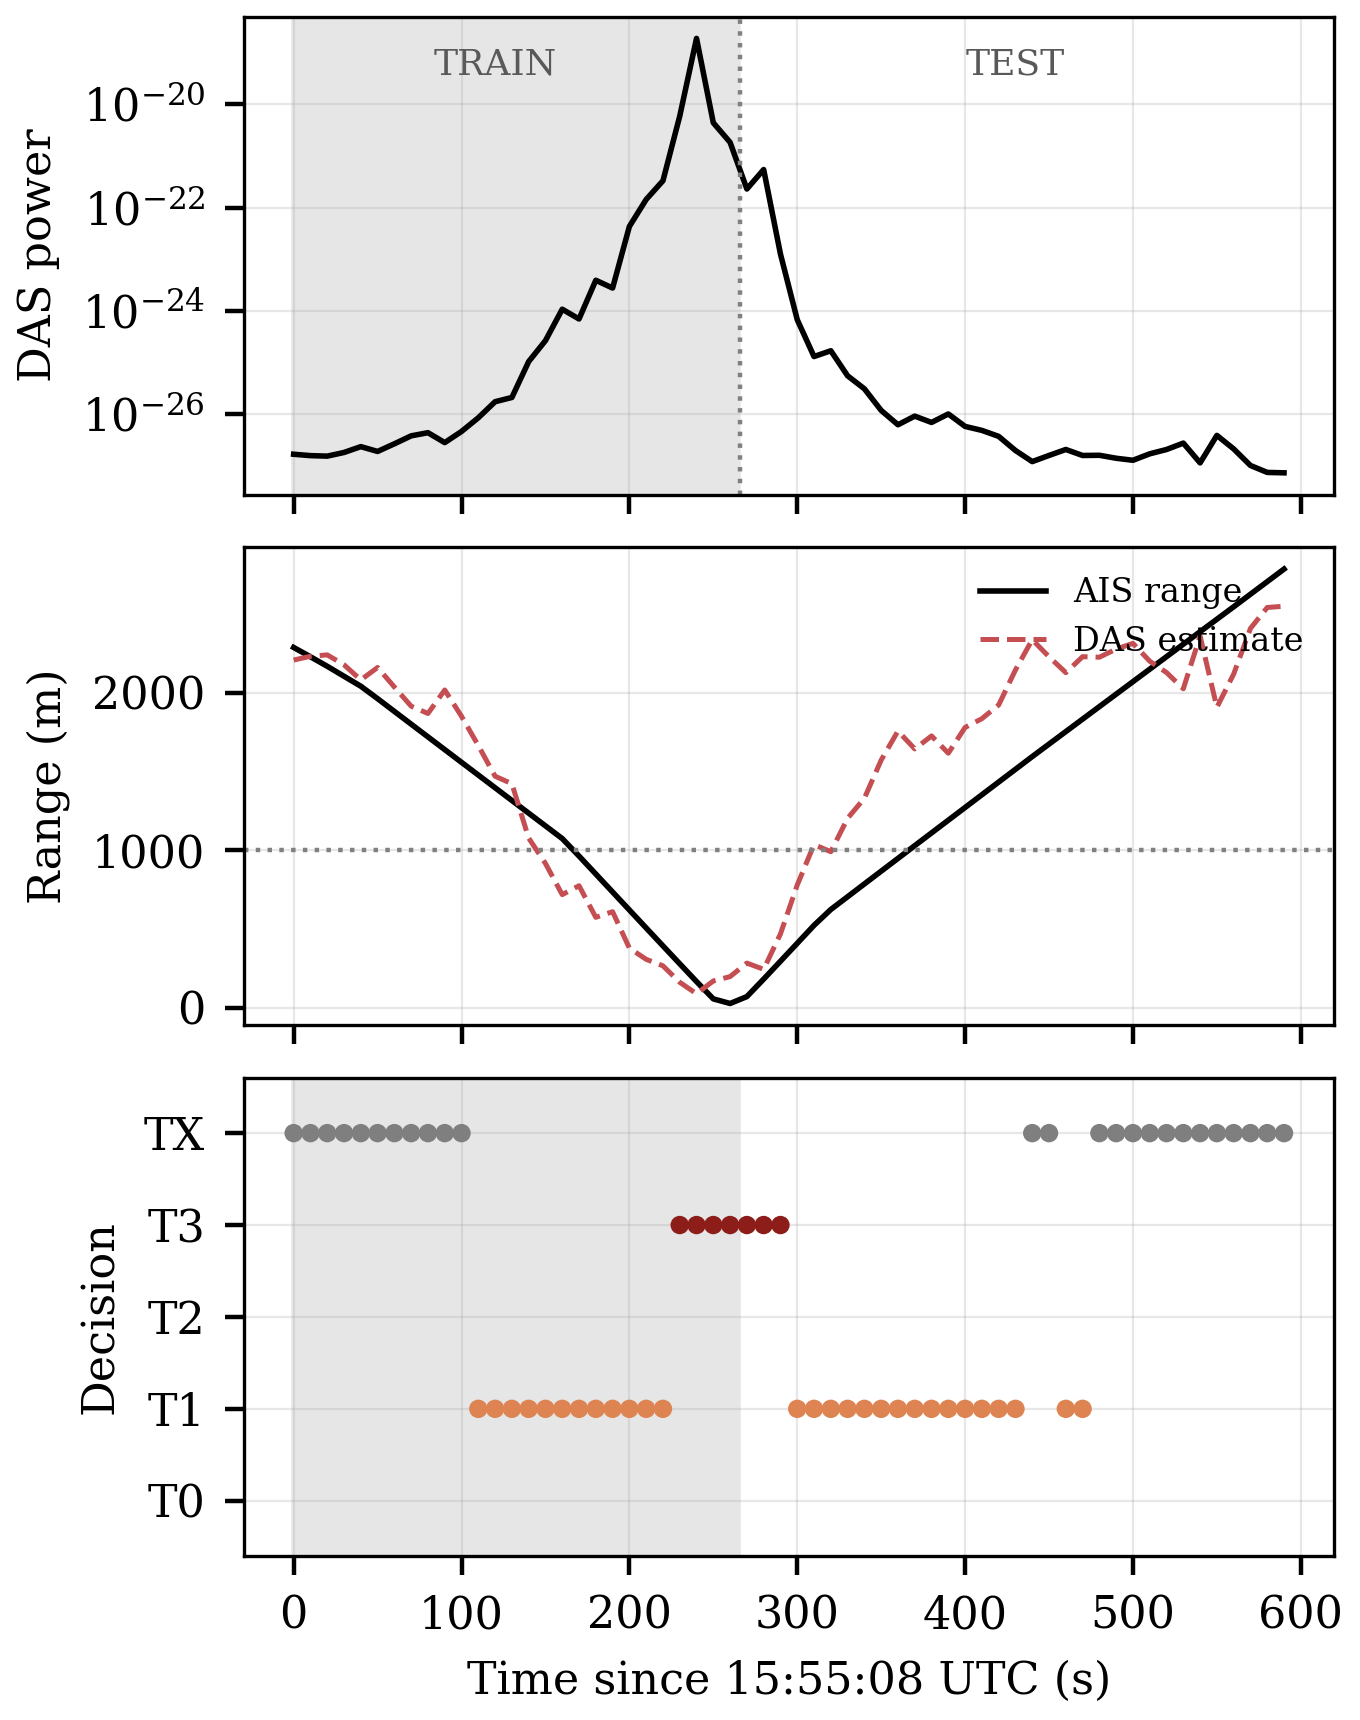
\includegraphics[width=0.45\textwidth]{figs/fig_transit.png}
\caption{Real transit response (Dataset A). Top: DAS window power spans seven orders of magnitude. Middle: AIS ground-truth range and independent DAS range inversion. Bottom: Graded decisions across the transit.}
\label{fig:transit}
\end{figure}

\subsection{Physical Detection on Real DAS}
\label{sec:detection-results}
Acoustic strain power correlates negatively with vessel distance at Spearman $\rho = -0.948$ ($p = 1.4\times10^{-30}$, $n=60$), confirming that measured seafloor acoustic energy scales monotonically with vessel proximity. Evaluated against corridor boundaries on the held-out leg, the coherent detection statistic yields the AUC values in Table~\ref{tab:auc}, reaching AUC $= 0.959$ (95\% CI $[0.887, 1.000]$) at a 1~km corridor threshold.

\begin{table}[!t]
\caption{DAS-Only Detection Performance on Held-Out Leg ($n=33$)}
\label{tab:auc}
\centering
\footnotesize
\begin{tabular}{@{}cccc@{}}
\toprule
Corridor $R_c$ & Positives ($n$) & AUC & 95\% Bootstrap CI \\
\midrule
200~m & 2 & 0.871 & [0.790, 0.952] \\
500~m & 4 & 0.897 & [0.828, 0.966] \\
1000~m & 10 & \textbf{0.959} & [0.887, 1.000] \\
\bottomrule
\end{tabular}
\end{table}

Fig.~\ref{fig:horizon} illustrates the physical detection boundary: coherent strain $Z_{\mathrm{coh}}$ remains above threshold $\tau_P = 7$ out to 1.5~km. Consequently, an uncorroborated physical detector triggers on passing ships well outside the security perimeter, resulting in 1.000 recall but only 0.526 precision (Table~\ref{tab:methods}).

\begin{figure}[!t]
\centering
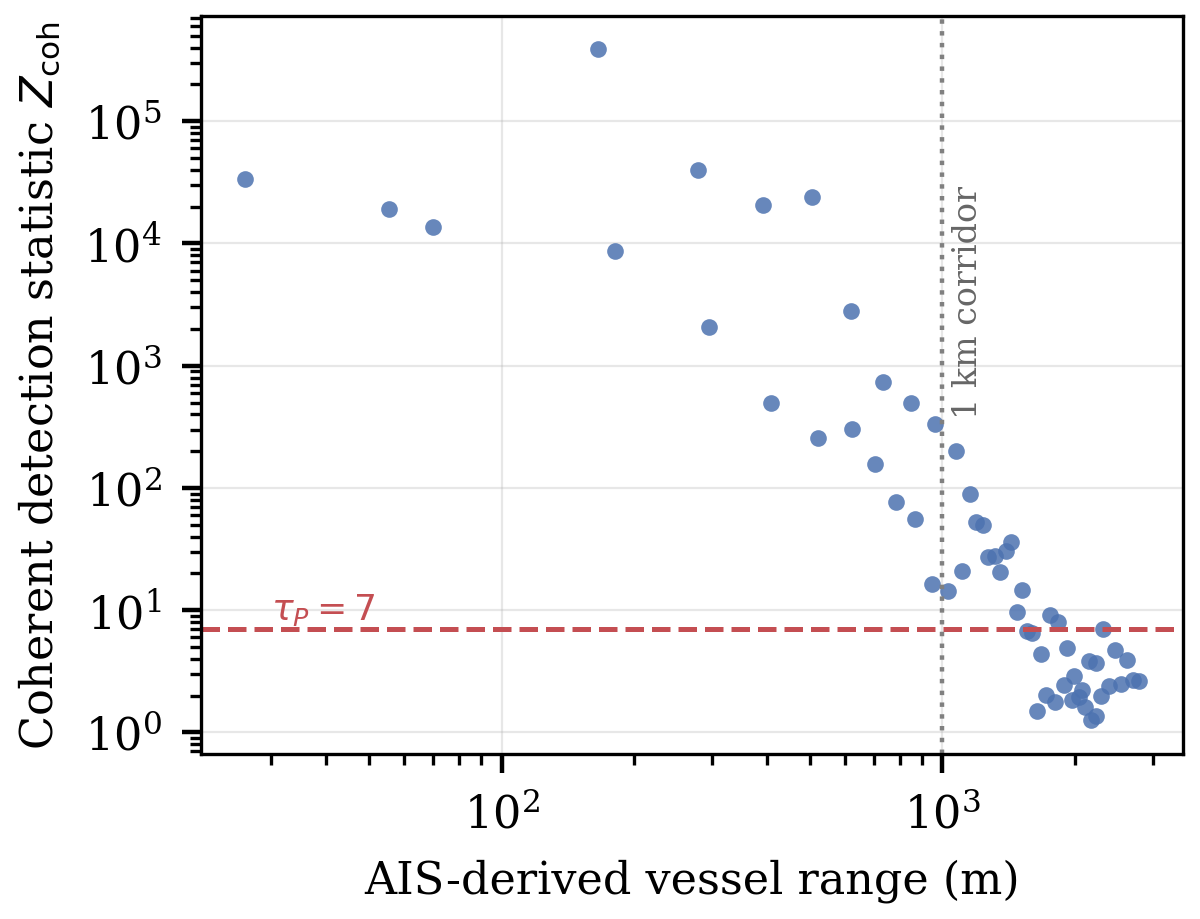
\includegraphics[width=0.42\textwidth]{figs/fig_horizon.png}
\caption{Coherent detection statistic against AIS range (Dataset A). The physical detection boundary extends to roughly 1.5~km, well outside the 1~km protection corridor.}
\label{fig:horizon}
\end{figure}

\subsection{Background Baseline and Threshold Calibration}
\label{sec:background}
On Dataset B, an unadapted static baseline drifts over 17 minutes, producing a 97.7\% detection exceedance rate. Implementing a rolling 200-second baseline stabilizes the statistic at a mean of 4.15 (p95 6.01, maximum 6.99). Sweeping $\tau_P$ identifies $\tau_P = 7$ as the minimal integer yielding zero background exceedances (Fig.~\ref{fig:far}). Operating the full decision engine across Dataset B (85 evaluated windows following 20-window baseline initialization) produced \dstate{TX} in 85/85 windows and zero false escalations to \dstate{T2}/\dstate{T3}, validating fail-closed behavior when vessel telemetry is absent. We distinguish these \emph{background false alarms} (detector exceedances on quiet seafloor) from \emph{environmental escalations} (T2/T3 decisions caused by natural hydrodynamic forcing) and \emph{vessel attribution errors} (misassigning responsibility).

\begin{figure}[!t]
\centering
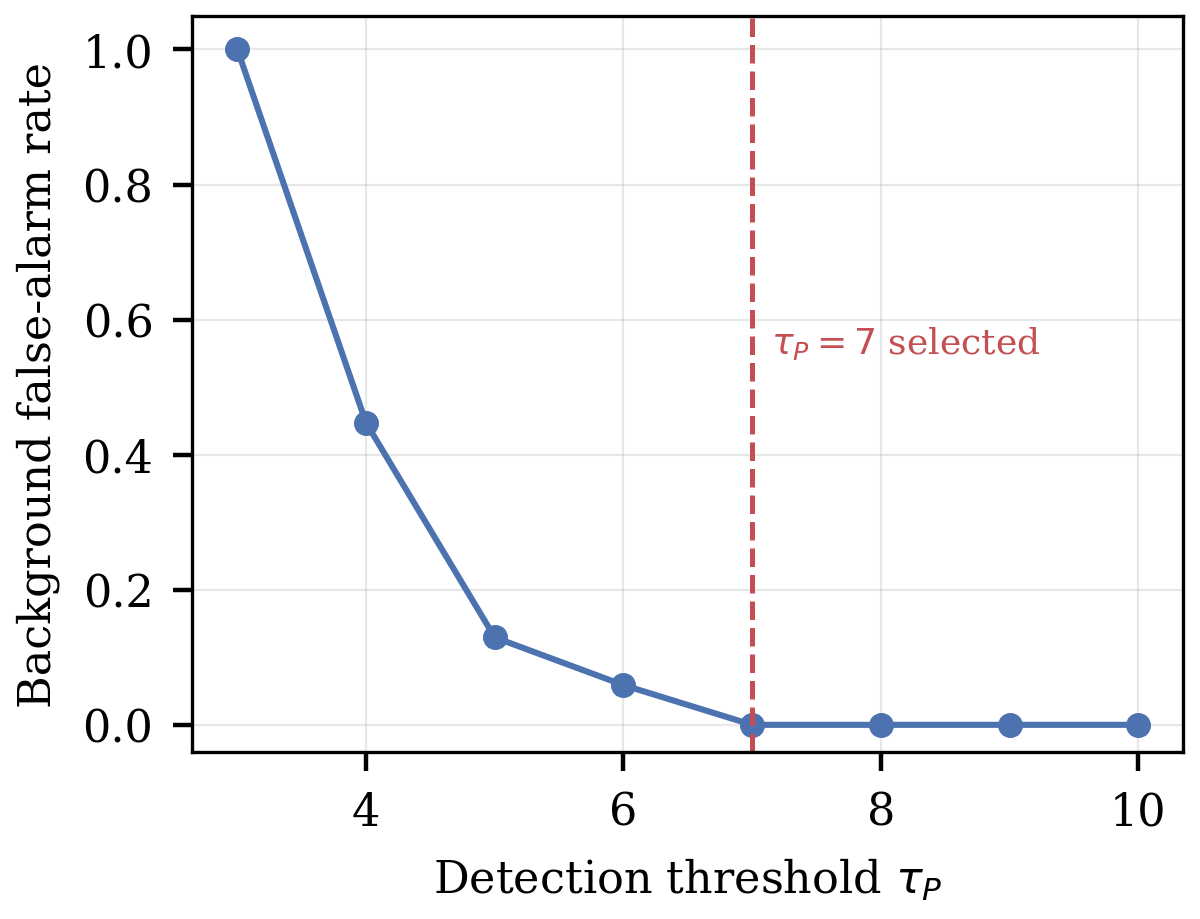
\includegraphics[width=0.42\textwidth]{figs/fig_far.png}
\caption{Background detection exceedance rate versus threshold on Dataset B (85 evaluated windows, rolling baseline). The reference threshold $\tau_P=3$ produces 100\% exceedances; $\tau_P=7$ achieves zero.}
\label{fig:far}
\end{figure}

\subsection{Independent Real-DAS Environmental Validation}
\label{sec:oliktok-results}

Dataset C provides an independent multi-week assessment of the physical detector under Arctic oceanographic conditions. Across 215 continuous hourly windows on 183 physical channels, the strain-rate field exhibited consistent seafloor coupling: mean integrated strain RMS was $550.85~\mathrm{nm/m/s}$ (median $553.59~\mathrm{nm/m/s}$), with spatial CV of 0.2349 and spatial Gini coefficient of 0.1265. Over the 27.625-day recording, temporal CV was 0.1239 with a negligible baseline drift slope of $+0.0188/\mathrm{hr}$ ($p = 0.8037$). Skewness and kurtosis were $+0.1547$ and $-1.1625$, respectively.

\begin{table}[!t]
\caption{Dryad Oliktok Real Submarine DAS Environmental Validation}
\label{tab:oliktok}
\centering
\footnotesize
\setlength{\tabcolsep}{3pt}
\begin{tabular}{@{}>{\raggedright\arraybackslash}p{0.33\columnwidth}>{\raggedright\arraybackslash}p{0.26\columnwidth}>{\raggedright\arraybackslash}p{0.33\columnwidth}@{}}
\toprule
Metric & Verified Value & Scientific Interpretation \\
\midrule
Recording Duration & 27.625~d (215~hr) & Continuous deployment (Aug 24--Sep 20, 2023) \\
Spatial Channels & 183 physical ch & Ch 1088--3672 (8.8--30.0~km offshore) \\
Integrated Strain RMS & 550.85~nm/m/s & Mean noise floor (median 553.59) \\
Skewness / Kurtosis & $+0.1547$ / $-1.1625$ & Sub-Gaussian seafloor strain distribution \\
Temporal Stability (CV) & 0.1239 & Stable multi-week acoustic baseline \\
Baseline Drift Slope & +0.0188 / hr & Negligible systematic sensor drift ($p=0.8037$) \\
Spatial CV / Gini & 0.2349 / 0.1265 & Homogeneous seafloor coupling \\
$\rho$ vs Wave Height ($H_s$) & +0.3141 ($p=2.63\times10^{-6}$) & Statistically significant wave coupling \\
$r$ vs Wave Height ($H_s$) & +0.3370 ($p=4.31\times10^{-7}$) & Linear wave height correlation \\
$\rho$ vs Pressure Variance & +0.4951 ($p=1.07\times10^{-14}$) & Hydrodynamic seafloor pressure tracking \\
$r$ vs Pressure Variance & +0.4903 ($p=2.11\times10^{-14}$) & Linear bottom pressure correlation \\
Quiet Baseline (\dstate{T0}) & 93 / 215 (43.26\%) & Classified as quiescent seafloor baseline \\
Uncorroborated (\dstate{T1}) & 122 / 215 (56.74\%) & Escalated to environmental disturbance \\
Corroborated (\dstate{T2}/\dstate{T3}) & 0 / 215 (0.0\%) & No T2/T3 vessel escalations occurred \\
Degraded Stream (\dstate{TX}) & 0 / 215 (0.0\%) & Zero unforced fail-closed triggers \\
\bottomrule
\end{tabular}
\end{table}

\begin{figure}[!t]
\centering
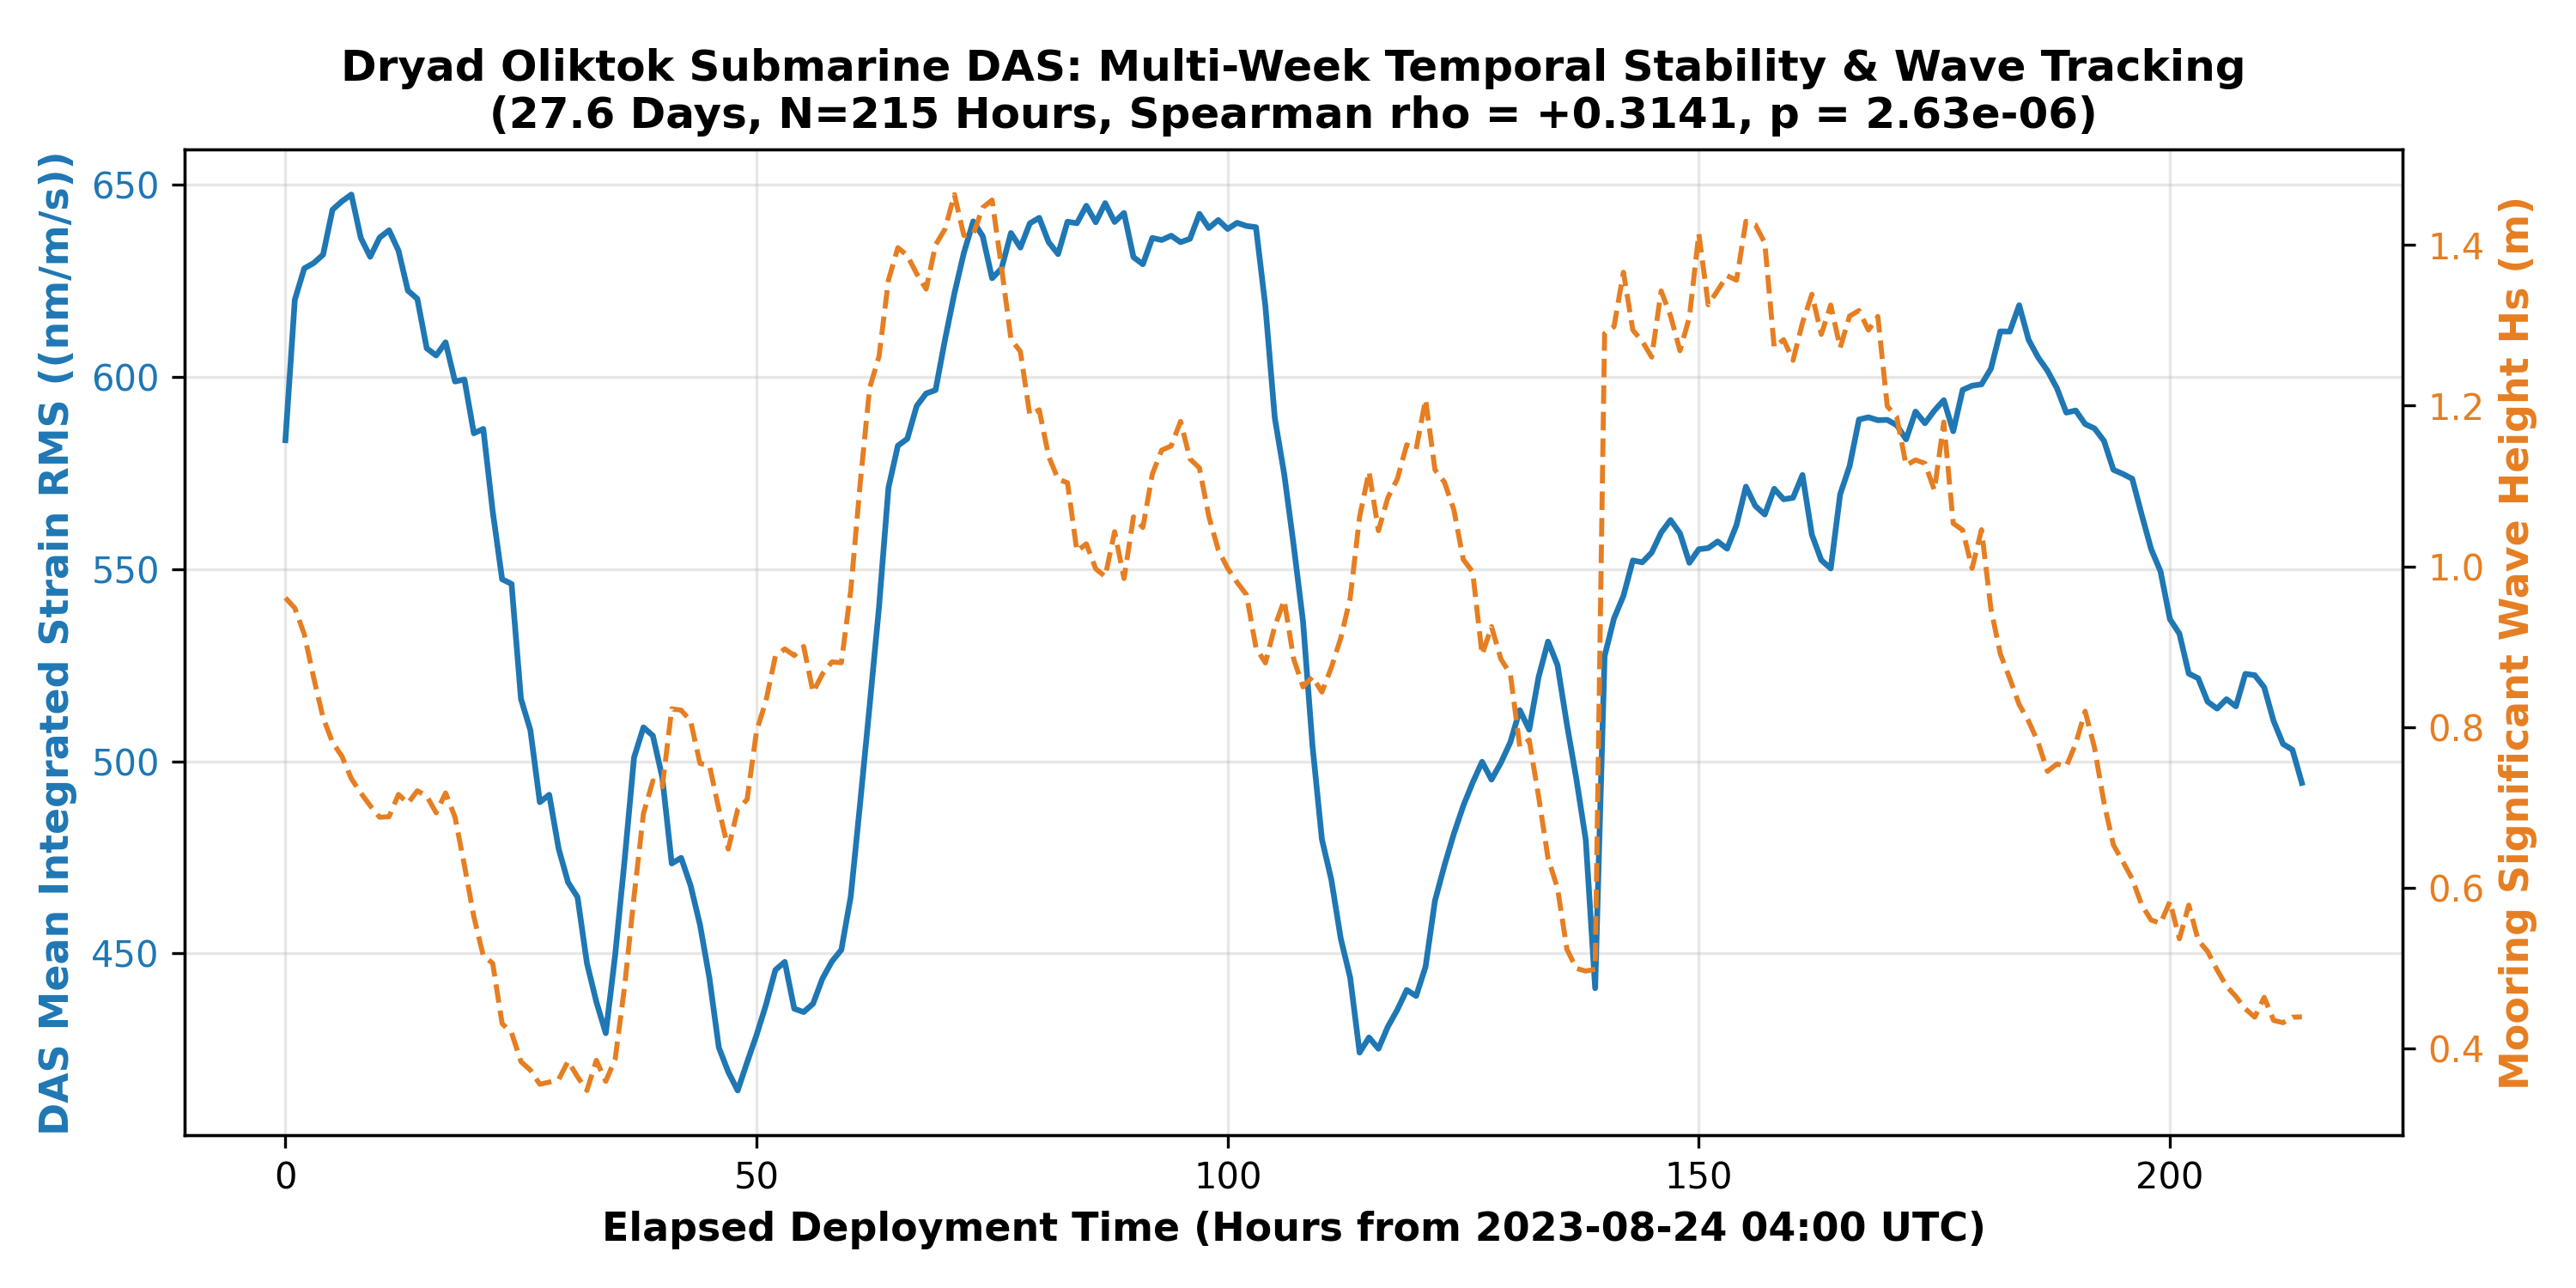
\includegraphics[width=0.45\textwidth]{figs/fig_oliktok_temporal.png}
\caption{Long-term temporal stability and environmental wave coupling on
Dataset C (Dryad Oliktok, 27.625 days). Seafloor acoustic energy tracks
independent ocean wave height without producing anomalous sensor drift.}
\label{fig:oliktok-temporal}
\end{figure}

The integrated strain exhibited statistically significant empirical associations
with independent oceanographic measurements: Spearman $\rho = +0.3141$
($p = 2.63\times10^{-6}$, Pearson $r = +0.3370, p = 4.31\times10^{-7}$) against
significant wave height $H_s$, and Spearman $\rho = +0.4951$
($p = 1.07\times10^{-14}$, Pearson $r = +0.4903, p = 2.11\times10^{-14}$) against
dynamic seafloor pressure variance. These correlations demonstrate empirical
monotonic association with surface hydrodynamics. They do not demonstrate
causal cable damage, as environmental records cannot establish causal physical
damage without annotated structural incident ground truth.

Processing Dataset C through the frozen decision pipeline produced 93
\dstate{T0} states (43.26\%) during calm periods, 122 \dstate{T1} states
(56.74\%) during wave excitation, and zero \dstate{T2}/\dstate{T3} states
(Table~\ref{tab:oliktok}). \textbf{No T2/T3 vessel-escalation decisions occurred
in the evaluated Oliktok environmental recording}, yielding an environmental
escalation rate of 0.0\%. Because Dataset C lacks vessel and AIS ground truth,
this finding is interpreted as an environmental robustness and false-escalation
avoidance observation rather than a vessel-attribution false-positive measurement.

\subsection{Decision Behavior on the Real Transit}
On the held-out transit leg of Dataset A ($n=33$), the decision hierarchy assigned 3 windows to \dstate{T3}, 16 to \dstate{T1}, and 14 to \dstate{TX} (Table~\ref{tab:states}). These state assignments correspond directly to physical proximity: confirmed escalation \dstate{T3} occurs at close approach (mean range 182.0~m, $C_P = 1.000, C_A = 0.738$); uncorroborated warning \dstate{T1} occurs at intermediate distances (mean range 1084.0~m, $C_P = 0.977, C_A = 0.191$); and degraded state \dstate{TX} occurs at distant ranges (mean range 2246.4~m) where acoustic energy drops toward the noise floor.

\begin{table}[!t]
\caption{Decision States on Held-Out Transit Leg ($n=33$)}
\label{tab:states}
\centering
\footnotesize
\begin{tabular}{@{}lccccc@{}}
\toprule
State & $n$ & Mean range (m) & $C_P$ & $C_A$ & $U$ \\
\midrule
\dstate{T3} & 3 & 182.0 & 1.000 & 0.738 & 0.094 \\
\dstate{T1} & 16 & 1084.0 & 0.977 & 0.191 & 0.361 \\
\dstate{TX} & 14 & 2246.4 & 0.096 & 0.066 & 0.225 \\
\bottomrule
\end{tabular}
\end{table}

\subsection{Method Comparison}
Table~\ref{tab:methods} compares the proposed framework against single-modality and partial fusion baselines on the held-out transit ($R_c = 1000$~m). All methods achieve a precision of 1.000 except the physical-only baseline (0.526).

\begin{table}[!t]
\caption{Method Comparison on Held-Out Transit Leg ($n=33$, $R_c=1000\,\mathrm{m}$)}
\label{tab:methods}
\centering
\footnotesize
\begin{tabular}{@{}lcccc@{}}
\toprule
Method & Accuracy & Precision & Recall & F1 \\
\midrule
behaviour\_only & 0.697 & 0.000 & 0.000 & 0.000 \\
physical + behaviour & 0.697 & 0.000 & 0.000 & 0.000 \\
physical-only & 0.727 & 0.526 & \textbf{1.000} & 0.690 \\
ais\_range\_only & 0.788 & 1.000 & 0.300 & 0.462 \\
association\_only & 0.788 & 1.000 & 0.300 & 0.462 \\
physical + spatial & 0.788 & 1.000 & 0.300 & 0.462 \\
physical + temporal & 0.849 & 1.000 & 0.500 & 0.667 \\
weighted (simple) & \textbf{0.909} & 1.000 & 0.700 & \textbf{0.824} \\
\textbf{Proposed (full)} & 0.788 & 1.000 & 0.300 & 0.462 \\
\bottomrule
\end{tabular}
\end{table}

The full proposed framework achieves F1 $= 0.462$, below simple weighted fusion (0.824) and physical + temporal association (0.667). Paired McNemar tests at $n=33$ indicate that performance differences between the proposed method and weighted fusion do not reach statistical significance ($p = 0.134$). The lower escalation F1 of the proposed framework stems directly from intentional conservatism: the decision hierarchy requires multi-channel agreement and low uncertainty before escalating, suppressing borderline or partially supported incursions to avoid false alarms.

\subsection{Ablation on Real Data}
Component ablation on the clean transit leg (Table~\ref{tab:ablation}) reveals that removing sensor health weighting, uncertainty modeling, or the adversarial consistency check leaves decision outputs unchanged. This behavior is consistent with design objectives: health gating, uncertainty divergence, and adversarial cross-checks activate under degraded or hostile conditions that are absent during an unperturbed transit. Their protective utility is demonstrated under active manipulation (Section~\ref{sec:adv-results}). Removing behavioral scoring increases F1 from 0.462 to 0.571 by lowering corroboration thresholds, whereas removing spatio-temporal association collapses F1 to 0.000, confirming that spatial and temporal gating provides the primary discriminative filter.

\begin{table}[!t]
\caption{Ablation Analysis on Held-Out Transit Leg ($n=33$)}
\label{tab:ablation}
\centering
\footnotesize
\begin{tabular}{@{}lccc@{}}
\toprule
Component Removed & Accuracy & Recall & F1 \\
\midrule
None (full proposed) & 0.788 & 0.300 & 0.462 \\
Sensor health weighting & 0.788 & 0.300 & 0.462 \\
Uncertainty model & 0.788 & 0.300 & 0.462 \\
Adversarial consistency check & 0.788 & 0.300 & 0.462 \\
Behavioral scoring & 0.818 & 0.400 & 0.571 \\
Spatio-temporal association & 0.697 & 0.000 & 0.000 \\
\bottomrule
\end{tabular}
\end{table}

\subsection{Adversarial Robustness and Evasion Rate}
\label{sec:adv-results}
To evaluate adversarial resilience, we perturbed the vessel-side AIS telemetry across 10 genuine incursion windows while leaving the physical fiber recording unaltered. Four attack families were tested across five severity levels (0.00, 0.25, 0.50, 0.75, 1.00): AIS range inflation, transponder suppression, timestamp manipulation, and combined multi-vector evasion (Table~\ref{tab:adv}).

\begin{table}[!t]
\caption{Adversarial Evaluation on Real DAS (10 Incursion Windows)}
\label{tab:adv}
\centering
\footnotesize
\begin{tabular}{@{}lccccc@{}}
\toprule
\multirow{2}{*}{Attack Family} & \multicolumn{5}{c}{Consistency-Check Firing Rate by Severity} \\
\cmidrule(l){2-6}
 & 0.00 & 0.25 & 0.50 & 0.75 & 1.00 \\
\midrule
AIS range inflation & 0.00 & 0.10 & 0.30 & 0.40 & 0.60 \\
Transponder suppression & 0.00 & 0.20 & 0.50 & 0.90 & 1.00 \\
Timestamp manipulation & 0.00 & 0.00 & 0.00 & 0.00 & 0.00 \\
Combined multi-vector & 0.00 & 0.30 & 0.70 & 0.90 & 1.00 \\
\midrule
AER (all families) & 0.00 & 0.00 & 0.00 & 0.00 & 0.00 \\
\bottomrule
\end{tabular}
\end{table}

The adversarial evasion rate (AER)---the proportion of true incursion trials that erroneously collapse to baseline \dstate{T0} under attack---was 0/200 (0.0) across all 20 evaluated conditions ($4\ \text{attack families} \times 5\ \text{severities}$, 10 incursion windows each). Within the evaluated vessel-side threat model, no incursion collapsed to \dstate{T0}. Mean uncertainty rose from 0.225 to 0.436 under maximum attack severity, and the range consistency check fired monotonically with attack strength for spatial falsifications (Fig.~\ref{fig:adversarial}). Importantly, this evaluation bounds vessel-side radio telemetry manipulation only; it does not represent resistance against physical optical fiber interference or interrogator firmware compromise.

\begin{figure}[t]
\centering
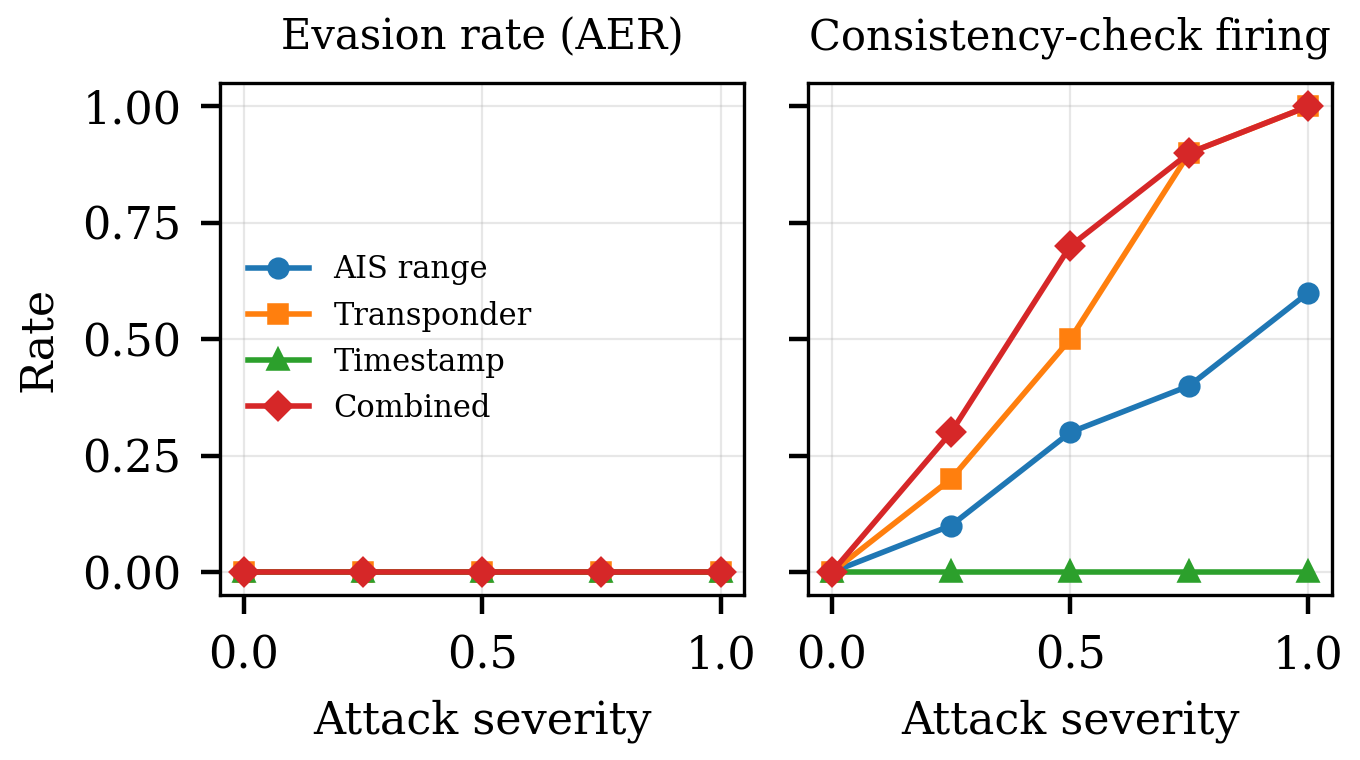
\includegraphics[width=\columnwidth]{figs/fig_adversarial.png}
\caption{Adversarial response on real DAS. Left: Adversarial evasion rate remains 0.0 across all severities. Right: Range consistency check fires monotonically for spatial attacks but remains inert under timestamp offsets.}
\label{fig:adversarial}
\end{figure}

\subsection{Robustness and Noise Sensitivity}
Under simulated optical channel dropout up to 90\%, escalation F1 remained stable at 0.462, while \dstate{TX} assignments increased from 42.4\% to 78.8\% and mean uncertainty rose from 0.279 to 0.485 (Fig.~\ref{fig:robustness}). This confirms graceful degradation: when sensing capacity is lost, the system flags degraded evidence rather than generating ungrounded classifications. In contrast, injecting extreme unmodeled Gaussian noise artificially inflated the fused reliability score $R$, indicating that severe noise excursions can shift windows out of \dstate{TX}.
unmodeled noise can displace windows from \dstate{TX}.

\begin{figure}[t]
\centering
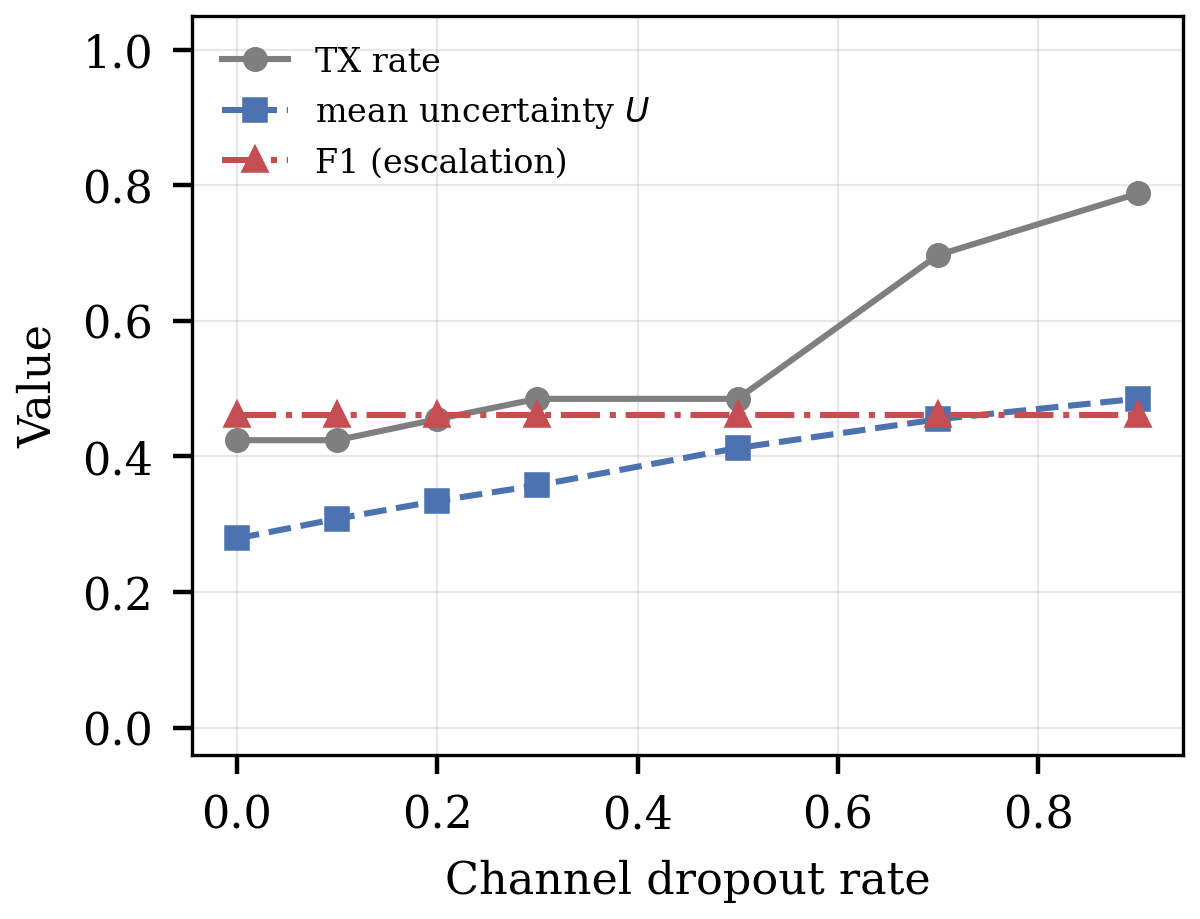
\includegraphics[width=0.95\columnwidth]{figs/fig_robustness.png}
\caption{Channel dropout robustness on real DAS. F1 remains constant while
\dstate{TX} declarations rise: the system degrades by asking for help, not by
guessing.}
\label{fig:robustness}
\end{figure}

\subsection{Calibration Assessment}
\label{sec:calibration}

\begin{figure}[t]
\centering
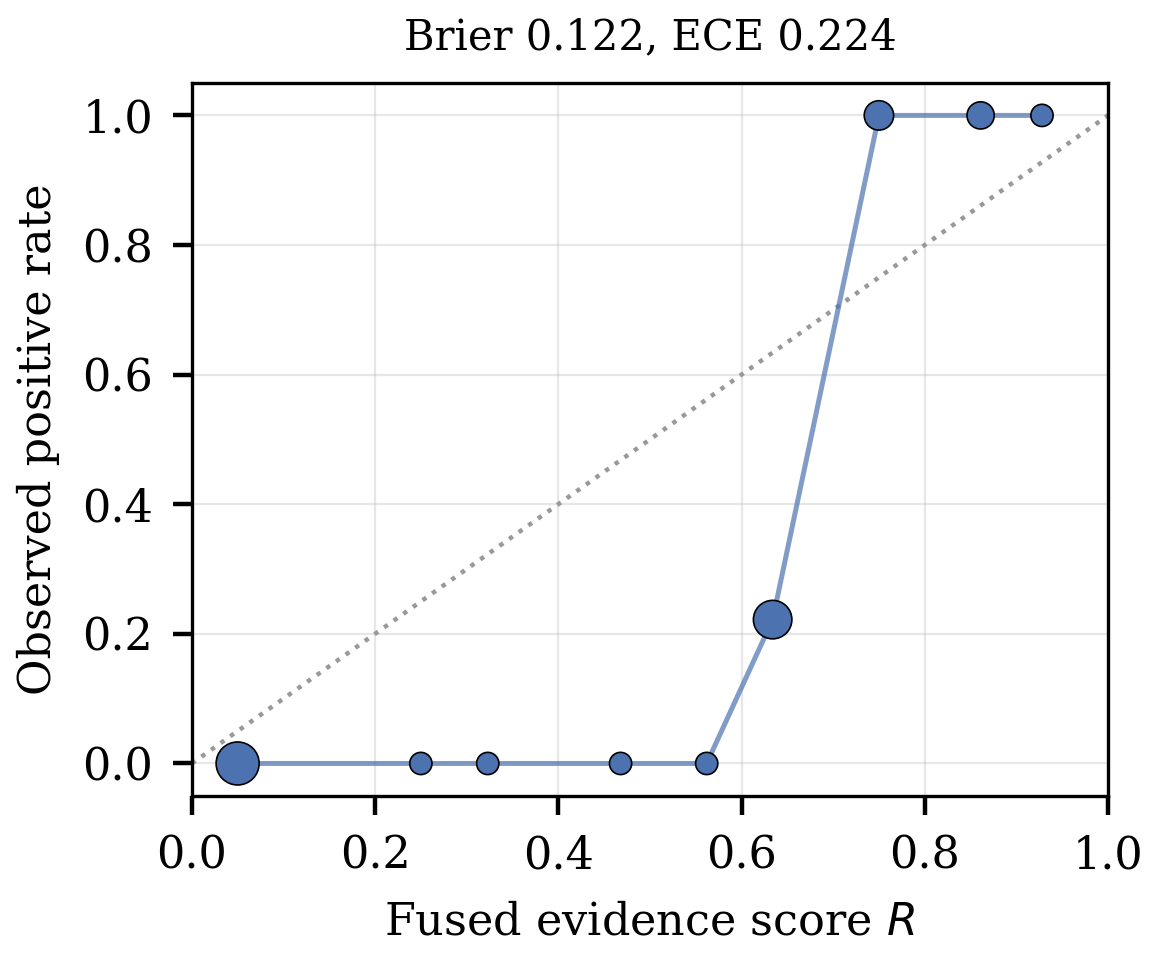
\includegraphics[width=0.95\columnwidth]{figs/fig_calibration.png}
\caption{Reliability calibration curve of fused score $R$ on the held-out
transit leg (Brier score $=0.122$; 10-bin expected calibration error (ECE)
$=0.224$). Marker area denotes bin sample occupancy.}
\label{fig:calibration}
\end{figure}

Evaluating the fused evidence score $R$ as a predicted probability yields a Brier score of 0.122 and a 10-bin Expected Calibration Error (ECE) of 0.224 on the held-out transit leg (Fig.~\ref{fig:calibration}). While $R$ orders events effectively (achieving high AUC), it displays overconfidence across intermediate probability bins (0.2--0.6). Fused score $R$ must therefore be interpreted as an operational ranking score rather than a calibrated posterior probability.

\subsection{Computational Performance}
\label{sec:performance}

\begin{table}[t]
\caption{Computational Latency (ms) and Throughput Profiling ($N=1{,}000$ Iterations)}
\label{tab:performance}
\centering
\setlength{\tabcolsep}{2pt}
\renewcommand{\arraystretch}{1.05}
\scriptsize
\begin{tabular}{@{}lrrrrr@{}}
\toprule
Stage & Mean & Median & P95 & Max & Throughput \\
\midrule
DAS Spectral Processing & 0.918 & 0.567 & 2.607 & 12.455 & 1{,}088.8~Hz \\
Spatio-Temporal Association & 0.031 & 0.020 & 0.051 & 2.147 & 32{,}083.4~Hz \\
Multimodal Evidence Fusion & 0.189 & 0.108 & 0.398 & 5.788 & 5{,}278.5~Hz \\
Decision State Machine & 0.009 & 0.005 & 0.010 & 2.564 & 111{,}271.8~Hz \\
\textbf{End-to-End Pipeline} & \textbf{8.289} & \textbf{6.230} & \textbf{19.526} & \textbf{63.437} & \textbf{120.6~Hz} \\
\bottomrule
\end{tabular}
\end{table}

Table~\ref{tab:performance} presents computational latency and throughput benchmarked across $N=1{,}000$ iterations on an Intel processor. End-to-end pipeline execution averages 8.289~ms (median 6.230~ms, p95 19.526~ms, throughput 120.6~Hz). Each constituent module operates with low overhead: DAS spectral processing averages 0.918~ms (1{,}088.8~Hz), spatio-temporal association averages 0.031~ms (32{,}083.4~Hz), multimodal evidence fusion requires 0.189~ms (5{,}278.5~Hz), and the decision state machine completes in 0.009~ms (111{,}271.8~Hz). All stages execute well within the 10-second real-time window cadence.

\section{Controlled Simulation Results}
\label{sec:sim}

To examine edge cases unrepresented in the real deployments---specifically sensor failure modes, multi-vessel tracking ambiguities, and conflicting counter-evidence---we evaluated 2{,}200 seeded simulation trials across 22 benchmark scenarios (S01--S22, 100 trials each). The framework produced 500 \dstate{T0}, 1{,}200 \dstate{T1}, 200 \dstate{T2}, 0 \dstate{T3}, and 300 \dstate{TX} decisions, corresponding to an accuracy of 0.4091 and an escalation F1 of 0.2353 (Table~\ref{tab:sim-baselines}).

\begin{table}[!t]
\caption{Comparative Evaluation Across 2,200 Controlled Simulation Trials}
\label{tab:sim-baselines}
\centering
\footnotesize
\setlength{\tabcolsep}{3pt}
\begin{tabular}{@{}lccccc@{}}
\toprule
Method & Acc. & Prec. & Recall & F1 & TX Rate \\
\midrule
physical-only & 0.3182 & 0.0000 & 0.0000 & 0.0000 & 0.0000 \\
association\_only & 0.3182 & 0.0000 & 0.0000 & 0.0000 & 0.1364 \\
behaviour\_only & 0.3182 & 0.0000 & 0.0000 & 0.0000 & 0.1364 \\
physical + temporal & 0.5909 & 1.0000 & 0.4000 & \textbf{0.5714} & 0.1364 \\
weighted fusion & 0.4545 & 1.0000 & 0.2000 & 0.3333 & 0.0000 \\
\textbf{Proposed (full)} & 0.4091 & 1.0000 & 0.1333 & 0.2353 & 0.1364 \\
\bottomrule
\end{tabular}
\end{table}

Component ablation under simulation shows physical-only detection achieving F1 $= 0.000$, physical + spatial association achieving F1 $= 0.4211$, physical + temporal association achieving F1 $= 0.5714$, and full fusion without health gating achieving F1 $= 0.3333$. Consistent with the empirical findings on real fiber, the proposed architecture trades unconstrained escalation recall to enforce fail-closed safety under sensor faults and uncorroborated alarms. These synthetic trials assess algorithmic response under controlled boundary conditions and cannot substitute for empirical in-situ validation.

\section{Discussion}

Synthesizing the empirical observations and controlled simulations leads to three primary findings:

First, the fail-closed safety principle is verified across authentic submarine optical records. Over 85 deep-sea background windows (EMSO) and 215 continuous Arctic environmental windows (Oliktok), the system produced zero false escalations to \dstate{T2}/\dstate{T3}. Under four vessel-side adversarial attack families evaluated on real DAS strain recordings, zero true incursion windows collapsed to unperturbed baseline \dstate{T0}.

Second, physical detection is empirically independent from causal attribution. Because acoustic vibrations propagate through sediment and water, large commercial vessels excite fiber strain channels out to 1.5~km. Physical-only monitoring triggers continuous false alarms during distant, benign navigation. Actionable infrastructure protection requires multi-channel spatio-temporal association and independent range verification.

Third, the lower escalation F1 scores ($0.462$ on real transit data, $0.235$ in simulation, evaluated independently) reflect a deliberate engineering design choice. The architecture prioritizes uncertainty quantification, health gating, and fail-closed safety over unconstrained recall.

\section{Limitations}
\label{sec:limitations}

\begin{enumerate}
\item \textbf{Absence of vessel ground truth in Oliktok:} Dataset C contains no vessel transponder logs or AIS data; its results validate environmental robustness and escalation avoidance, not vessel classification accuracy.
\item \textbf{Absence of causal cable damage ground truth:} No dataset contains verified structural cable damage incidents; attribution claims cannot be causally verified against physical breaks.
\item \textbf{1D proximity constraint in Marlinks:} Dataset A provides 1D distance $y$ rather than complete 2D geographic coordinates or polyline geometry.
\item \textbf{Unresolved non-vessel mechanical disturbances ($H_3$):} Distinguishing vessel anchoring from benthic dredging or geological motion remains unvalidated on real submarine fiber.
\item \textbf{Non-interchangeability of simulation and real data:} Synthetic simulation provides controlled edge cases but cannot substitute for in-situ oceanographic propagation.
\item \textbf{Vessel-side adversarial scope:} The threat model is restricted to AIS telemetry falsification and does not cover physical fiber tampering, optical interrogator compromise, or network eavesdropping.
\item \textbf{Hardware prototype boundary:} Benchtop hardware validation is not equivalent to submerged maritime deployment.
\item \textbf{Frequency-domain DAS limitations:} Processed spectral band powers do not equal full-bandwidth high-frequency optical phase waveforms.
\item \textbf{Correlation versus causation:} Oceanographic wave correlations demonstrate natural hydrodynamic coupling, not causal cable degradation.
\item \textbf{Geographic diversity limitations:} Validated data represent three localized regions (North Sea, Ionian Sea, Beaufort Sea), which do not encompass global variations in seabed geology, water depth, and maritime traffic.
\end{enumerate}

\section{Reproducibility}

All reported results derive deterministically from frozen code and data manifests. Source files are verified through cryptographic SHA-256 hashes: Dataset A (\texttt{46f5d2838342}), Dataset B (\texttt{8af2afac41b9}), Dataset C (\texttt{5fa69e4cf90a}), and the companion along-cable file (\texttt{6f9927adbfea}). Pseudo-random number generators use fixed seed 42. Experiments are replicated via \texttt{scripts/run\_real\_evaluation.py} and \texttt{scripts/run\_phase3\_validation.py}. No reported metric was manually altered.

\section{Conclusion and Future Work}
\label{sec:conclusion}

This paper presented an uncertainty-aware multimodal evidence fusion framework for assessing vessel-associated subsea cable disturbances. Evaluated across three real submarine DAS records spanning the North Sea, Mediterranean, and Arctic Ocean, the framework demonstrates that physical disturbance detection must be decoupled from vessel association and causal attribution. Across 27.6 days of Arctic environmental recording and 1{,}050~s of deep-sea baseline data, the system produced zero false escalations to \dstate{T2}/\dstate{T3}, while maintaining an adversarial evasion rate of 0.0 against vessel-side AIS manipulation. Security claims are bounded to the evaluated threat model, escalation F1 is documented alongside unconstrained baselines, and all results remain grounded in verifiable artifacts.

\subsection{Future Work: Hardware Validation Scope}
\label{sec:hardware}

The physical ESP32--MPU6050 testbed described in early project plans was not constructed; no hardware metrics appear in this paper. We formalize its experimental scope for future reproducibility.

\textbf{Configuration:} Five ESP32 microcontrollers paired with MPU6050 six-axis inertial measurement units (IMUs) sampled at 10~Hz, deployed along a scaled conduit in a hydrodynamic test tank, communicating over Wi-Fi/LoRa to an edge aggregator running the decision engine.

\textbf{Intended Measurements:} (i) Real-world communication packet loss and radio latency; (ii) physical sensor disconnects and saturation faults; and (iii) empirical verification of edge decision execution under electrical noise.

\textbf{Claim Boundaries:} A benchtop IMU testbed cannot validate ocean acoustic propagation or deep-sea vessel dynamics; it serves strictly to test embedded firmware execution under controllable physical hardware faults.

\begin{thebibliography}{00}
\bibitem{b1} N. Srikanth and S. S. Rao, ``Subsea cable health monitoring system,'' in \textit{Proc. IEEE Asian Conf. Energy, Power Transp. Electrific. (ACEPT)}, 2017, doi: 10.1109/ACEPT.2017.8168582.
\bibitem{b2} A. Tudorache, J. Timmerberg, S. Mylvaganam, M. Stender, F. Xiaozhong, and L. Zhu, ``Subsea cable tracking using data fusion of signals from array of sensing coils,'' in \textit{Proc. 30th Annu. Conf. Eur. Assoc. Educ. Electr. Inf. Eng. (EAEEIE)}, 2021, doi: 10.1109/EAEEIE50507.2021.9530924.
\bibitem{b3} A. P. Balasuriya and T. Ura, ``Autonomous underwater vehicles for submarine cable inspection: Experimental results,'' in \textit{Proc. IEEE Int. Conf. Syst., Man, Cybern. (SMC)}, 2001, doi: 10.1109/ICSMC.2001.969841.
\bibitem{b4} W. Tang, D. Flynn, and V. Robu, ``Sensing technologies and artificial intelligence for subsea power cable asset management,'' in \textit{Proc. IEEE Int. Conf. Prognostics Health Manage. (ICPHM)}, 2021, doi: 10.1109/ICPHM51084.2021.9486586.
\bibitem{b11} E. E. Ramirez-Torres \textit{et al.}, ``Vessel Detection and Localization Using Distributed Acoustic Sensing in Submarine Optical Fiber Cables,'' \textit{IEEE J. Sel. Topics Appl. Earth Observ. Remote Sens.}, 2026, doi: 10.1109/JSTARS.2026.3716768.
\bibitem{b12} E. E. Ramirez-Torres \textit{et al.}, ``Marlinks-NS DAS: Dataset for Vessel Detection and Distance Estimation Using Distributed Acoustic Sensing in Submarine Optical Fiber Cables,'' Zenodo, 2026, doi: 10.5281/zenodo.15611778.
\bibitem{b13} E. E. Ramirez-Torres \textit{et al.}, ``A Distributed Acoustic Sensing Dataset for Vessel Detection and Localization in Submarine Cable Protection,'' arXiv:2607.28306, 2026, doi: 10.48550/arXiv.2607.28306.
\bibitem{b14} L. Thiem, M. Vaupel, S. Wienecke, J. Eidsvik, K. Taweesintananon, and M. Landr{\o}, ``Tracking ships with submarine cables: Unsupervised arrival time detection and event localization using distributed acoustic sensing,'' Zenodo, 2026, doi: 10.5281/zenodo.18851481.
\bibitem{b15} J. Davis \textit{et al.}, ``Distributed acoustic sensing observations of ocean surface waves and seafloor pressure in the Arctic,'' Dryad Digital Repository, 2024, doi: 10.5061/dryad.brv15dvnz.
\bibitem{b5} P. Prasad, V. Vatsal, and R. Roy Chowdhury, ``Maritime Vessel Route Extraction and Automatic Information System (AIS) Spoofing Detection,'' in \textit{2021 Int. Conf. Advances in Electrical, Computing, Communication and Sustainable Technologies (ICAECT)}, 2021, doi: 10.1109/ICAECT49130.2021.9392536.
\bibitem{b6} E. d'Afflisio, P. Braca, and P. Willett, ``Malicious AIS spoofing and abnormal stealth deviations: A comprehensive statistical framework for maritime anomaly detection,'' \textit{IEEE Trans. Aerosp. Electron. Syst.}, vol. 57, no. 5, pp. 3151--3165, 2021, doi: 10.1109/TAES.2021.3090715.
\bibitem{b7} J. Coleman, F. Kandah, and B. Huber, ``Behavioral Model Anomaly Detection in Automatic Identification Systems (AIS),'' in \textit{2020 10th Annual Computing and Communication Workshop and Conference (CCWC)}, 2020, pp. 481--487.
\bibitem{b8} Z. Deng and J. Wang, ``A Novel Evidence Conflict Measurement for Multi-Sensor Data Fusion Based on the Evidence Distance and Evidence Angle,'' \textit{Sensors}, vol. 20, no. 2, p. 381, 2020, doi: 10.3390/s20020381.
\bibitem{b9} F. Xiao and B. Qin, ``A Weighted Combination Method for Conflicting Evidence in Multi-Sensor Data Fusion,'' \textit{Sensors}, vol. 18, no. 5, p. 1487, 2018, doi: 10.3390/s18051487.
\bibitem{b10} Q. Liang, Z. Liu, and Z. Chen, ``A Networked Method for Multi-Evidence-Based Information Fusion,'' \textit{Entropy}, vol. 25, no. 1, p. 69, 2023.
\end{thebibliography}

\end{document}
